\documentclass{article}% use option titlepage to get the title on a page of its own.

\title{Tutorial k-Nearest Neighbours Regression}
\date{2020\\ August}
\author{Marcos del Cueto}

\usepackage{amsmath}
\usepackage{mathtools}
\usepackage{float}
\usepackage{listings}
\usepackage{color}
\usepackage{xcolor}
\usepackage[a4paper, portrait, margin=2cm]{geometry}
\renewcommand{\floatpagefraction}{.8}%
\definecolor{lightgrey}{rgb}{0.9,0.9,0.9}
\definecolor{darkgreen}{rgb}{0,0.6,0}
\begin{document}
\maketitle
\section{Introduction}

In the last years, there has been an explosion on machine learning (ML) tools that make their use much more affordable to users. However, a risk of such advancements is that it is easier to treat the ML tools as a black box. I have seen several online tutorials dealing with k-nearest neighbours (k-NN) classification. However, one must remember that k-NN can also be used as a regression tool, to estimate values of a continuous target property. Given how extended the use of regression methods are in all branches of science, I am surprised there are no more tutorials of such a basic (yet useful) method as k-NN regression.

\paragraph{Goals tutorial.} I have prepared this short tutorial as a direct way to:
\begin{itemize}
	\item Provide simple example on how to prepare data for regression.
	\item Show how to perform k-NN regression and optimize k.
	\item Exemplify how k-NN regression works.
	\item Show how different weight functions can affect k-NN prediction.
	\item Discuss some limitations of k-NN regression.
\end{itemize}

\paragraph{Classification vs regression}

\paragraph{Python and scikit-learn}

\section{Generate data}
To simplify things here, we will consider here a one-dimensional dataset. This means that we have only one descriptor (aka feature) $\mathbf{x}$, and a target property $f(\textbf{x})$. As a generic example, I am going to use in this tutorial a small database formed by ten points that follow the function:

\begin{align}
    f(x) = e^{x}
	\label{eqn:exp}
\end{align}

The points considered in this example are shown in Table \ref{tab:dataset}, as well as in Figure \ref{fig:Fig1}.

\begin{table}[h!]
	\begin{center}
		\caption{Caption}
		\label{tab:dataset}
		\begin{tabular}{l|c|r} % <-- Alignments: 1st column left, 2nd middle and 3rd right, with vertical lines in between
			$x_n$ & $f(x_n)$\\
			\hline
				5.00 & 148.41\\
				5.20 & 181.27\\
				5.40 & 221.41\\
				5.60 & 270.43\\
				5.80 & 330.30\\
				6.00 & 403.43\\
				6.20 & 492.75\\
				6.40 & 601.85\\
				6.60 & 735.10\\
				6.80 & 897.85\\
		\end{tabular}
	\end{center}
\end{table}

\begin{figure*}[!htbp]
	\centering
	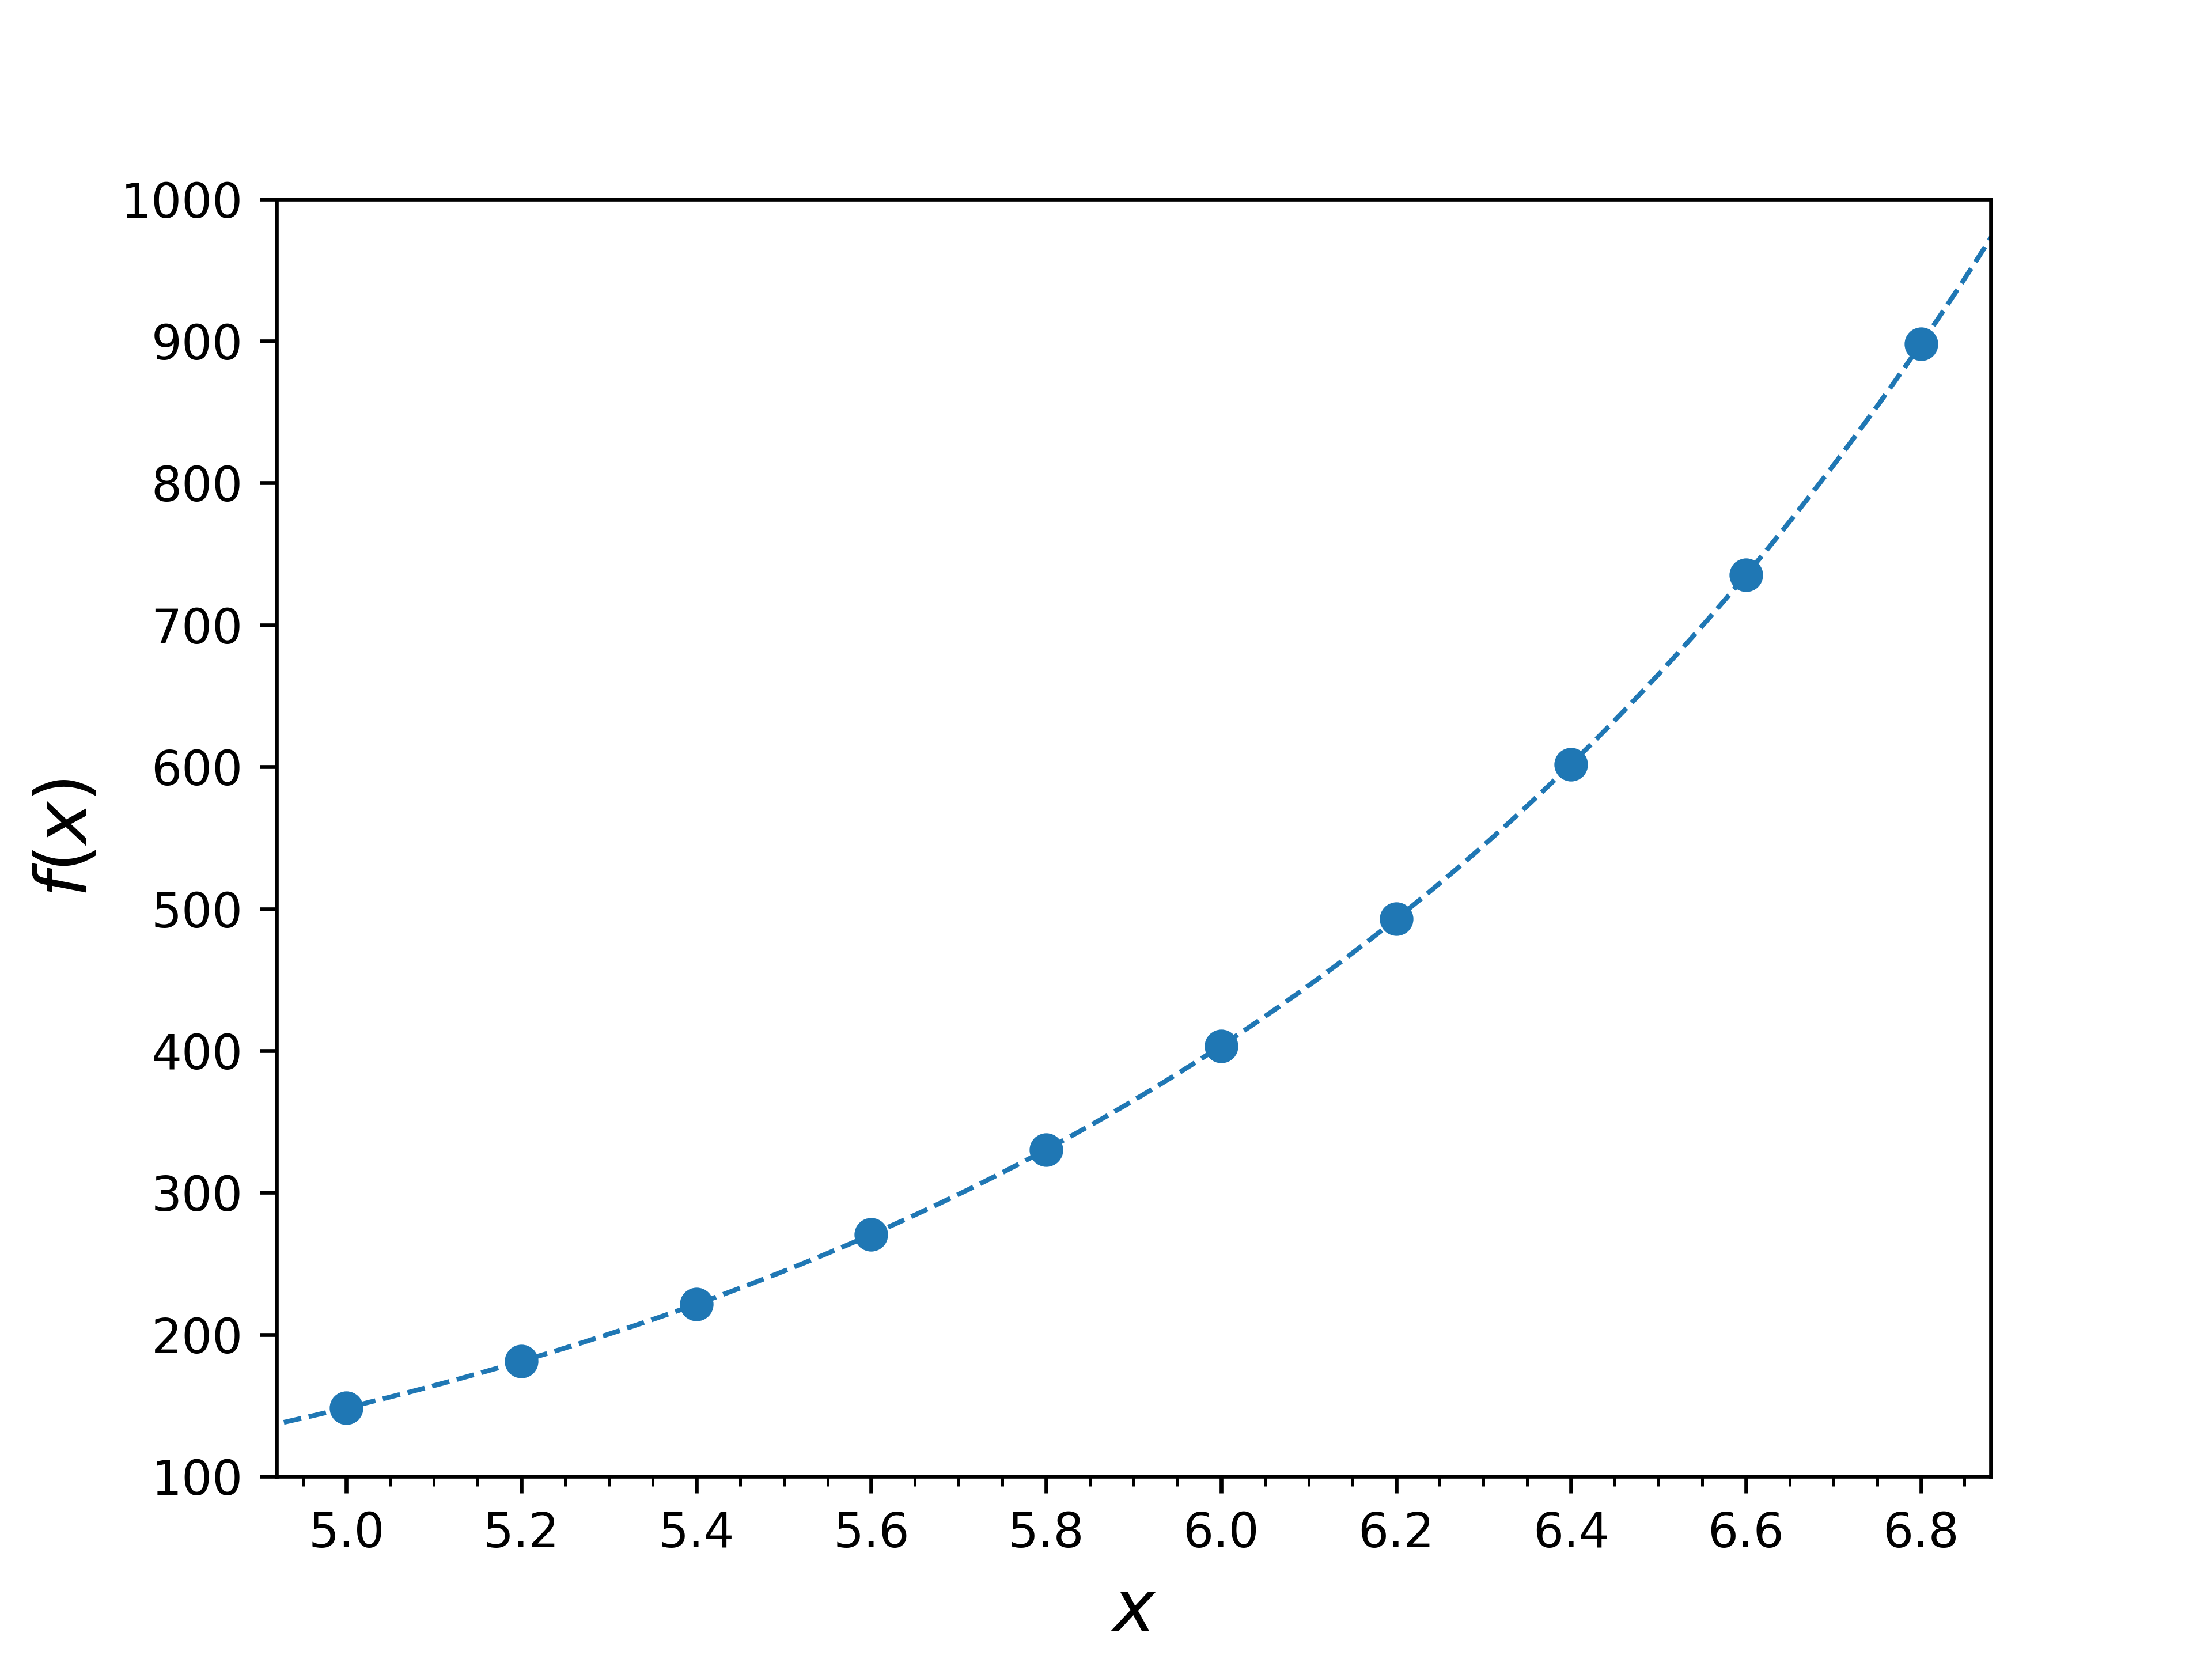
\includegraphics[width=0.75\textwidth]{figures/Fig1.png}
	\caption{Caption.}
	\label{fig:Fig1}
\end{figure*}

I show now the code used to generate this dataset, as well as Figure \ref{fig:Fig1}.

\begin{lstlisting}[language=Python, caption=Code1,backgroundcolor=\color{lightgrey},keywordstyle=\color{darkgreen},commentstyle=\color{red},
showspaces=false,numbers=left,stringstyle=\color{purple}]
import math
import matplotlib.pyplot as plt 
from matplotlib.ticker import (MultipleLocator)
import numpy as np

### 1) Generate data
list_x = []
list_y = []
for i in np.arange(5, 7, 0.2):
    x = i 
    y = math.exp(x)
    list_x.append(x)
    list_y.append(y)
    print("%.2f,%.6f" %(x, y)) 
list_x = np.array(list_x).reshape(-1, 1)
list_y = np.array(list_y)
basic_x = np.arange(4.9, 7.0, 0.01)
basic_y = [math.exp(x) for x in basic_x]
# Plot graph
plt.plot(basic_x,basic_y,color='C0',linestyle='dashed',linewidth=1)
plt.scatter(list_x, list_y,color='C0')
plt.xlabel('$x$',fontsize=15)
plt.ylabel('$f(x)$',fontsize=15)
plt.xticks(np.arange(5,7,0.2))
plt.xlim(4.92,6.88)
plt.ylim(100,1000)
axes = plt.gca()
axes.xaxis.set_minor_locator(MultipleLocator(0.05))
# Save plot into png
file_name='Fig1.png'
plt.savefig(file_name,format='png',dpi=600)
plt.close()
\end{lstlisting}


\section{Data analysis}
With k-NN regression, the $y$ value at any given $\mathbf{x}$ configuration is given as an average of nearby neighbours. When using this algorithm, one has to select two main parameters:
\begin{enumerate}
	\item How many near neighbours are considered
	\item How the average of the neighbours is calculated
\end{enumerate}

\subsection{Cross-validation to optimize k}
Regarding the first of these points, a simple method to select the optimum number of k nearest neighbours to make accurate predictions is to use a grid search. A grid search involves trying different k values and finally choosing the one that minimizes the prediction error. As with any ML model, one is faced with the task of how to select the data that will be used to train the model and the data that will be used to test the model accuracy. Since we have a small amount of data here, we will use the leave-one-out (LOO) cross-validation (for more complex datasets, one may opt for a k-fold cross-validation).

I am not going to go into the details of LOO, but for a dataset with $N$ samples, one trains the ML model with $N-1$ points, and use the remaining point as a test. This procedure is repeated $N$ times, so each point is used exactly once as a test (see Figure X). As a result, one ends with a predicted value for each point. Then, the predicted value of each point is compared with its actual value. As an error metric, we have used the root mean square error (rmse) here. Finally, we can compare the (rmse) obtained for different k values, and select as an optimum value the one that minimizes the rmse.

Here I provide the code necessary to do this:
\begin{lstlisting}[language=Python, caption=Code2,backgroundcolor=\color{lightgrey},keywordstyle=\color{darkgreen},commentstyle=\color{red},
showspaces=false,numbers=left,stringstyle=\color{purple}]
import math
import matplotlib.pyplot as plt 
import numpy as np
from sklearn import preprocessing
from sklearn.model_selection import LeaveOneOut
from sklearn.metrics import mean_squared_error
from sklearn import neighbors
from matplotlib.ticker import (MultipleLocator)

### 1) Generate data
list_x = []
list_y = []
for i in np.arange(5, 7, 0.2):
x = i 
y = math.exp(x)
list_x.append(x)
list_y.append(y)
list_x = np.array(list_x).reshape(-1, 1)
list_y = np.array(list_y)
basic_x = np.arange(4.9, 7.0, 0.01)
basic_y = [math.exp(x) for x in basic_x]
### 2) Leave one out
best_rmse = 0 
best_k = 0 
possible_k = [1,2,3,4,5,6,7,8,9]
for k in possible_k:
y_pred = []
x_pred = []
X = np.array(list_x).reshape(-1, 1)
validation=LeaveOneOut().split(X)
for train_index, test_index in validation:
X_train, X_test = list_x[train_index], list_x[test_index]
y_train, y_test = list_y[train_index], list_y[test_index]
# scale data
scaler = preprocessing.StandardScaler().fit(X_train)
X_train_scaled = scaler.transform(X_train)
X_test_scaled = scaler.transform(X_test)
knn = neighbors.KNeighborsRegressor(n_neighbors=k, weights='uniform')
pred = knn.fit(X_train_scaled, y_train).predict(X_test_scaled)
y_pred.append(pred)
x_pred.append(X_test)
mse = mean_squared_error(y_pred,list_y)
rmse = np.sqrt(mse)
print('k: %i, RMSE: %.2f' %(k, rmse))
if rmse < best_rmse or k==possible_k[0]:
best_rmse = rmse
best_k = k 
print("Optimum: kNN, k=%i, RMSE: %.2f" %(best_k,best_rmse))
\end{lstlisting}

The output of the code above is:
\begin{lstlisting}[backgroundcolor=\color{lightgrey}]
k: 1, RMSE: 95.55
k: 2, RMSE: 74.87
k: 3, RMSE: 105.13
k: 4, RMSE: 122.74
k: 5, RMSE: 152.07
k: 6, RMSE: 173.34
k: 7, RMSE: 202.04
k: 8, RMSE: 230.51
k: 9, RMSE: 264.38
Optimum: kNN, k=2, RMSE: 74.87
\end{lstlisting}

We can use this optimum case, with k=2, to visualize how the k-NN regression algorithm is working. In Figure \ref{fig:Fig2}, we show how, when trying to predict the value of $x_0$, the predicted value $x_0'$ is calculated as the average of its nearest neighbours, $x_1$ and $x_2$; $x_1'$ is predicted as the average of its two nearest neighbours, $x_0$ and $x_2$ and so on.

\begin{figure*}[!htbp]
	\centering
	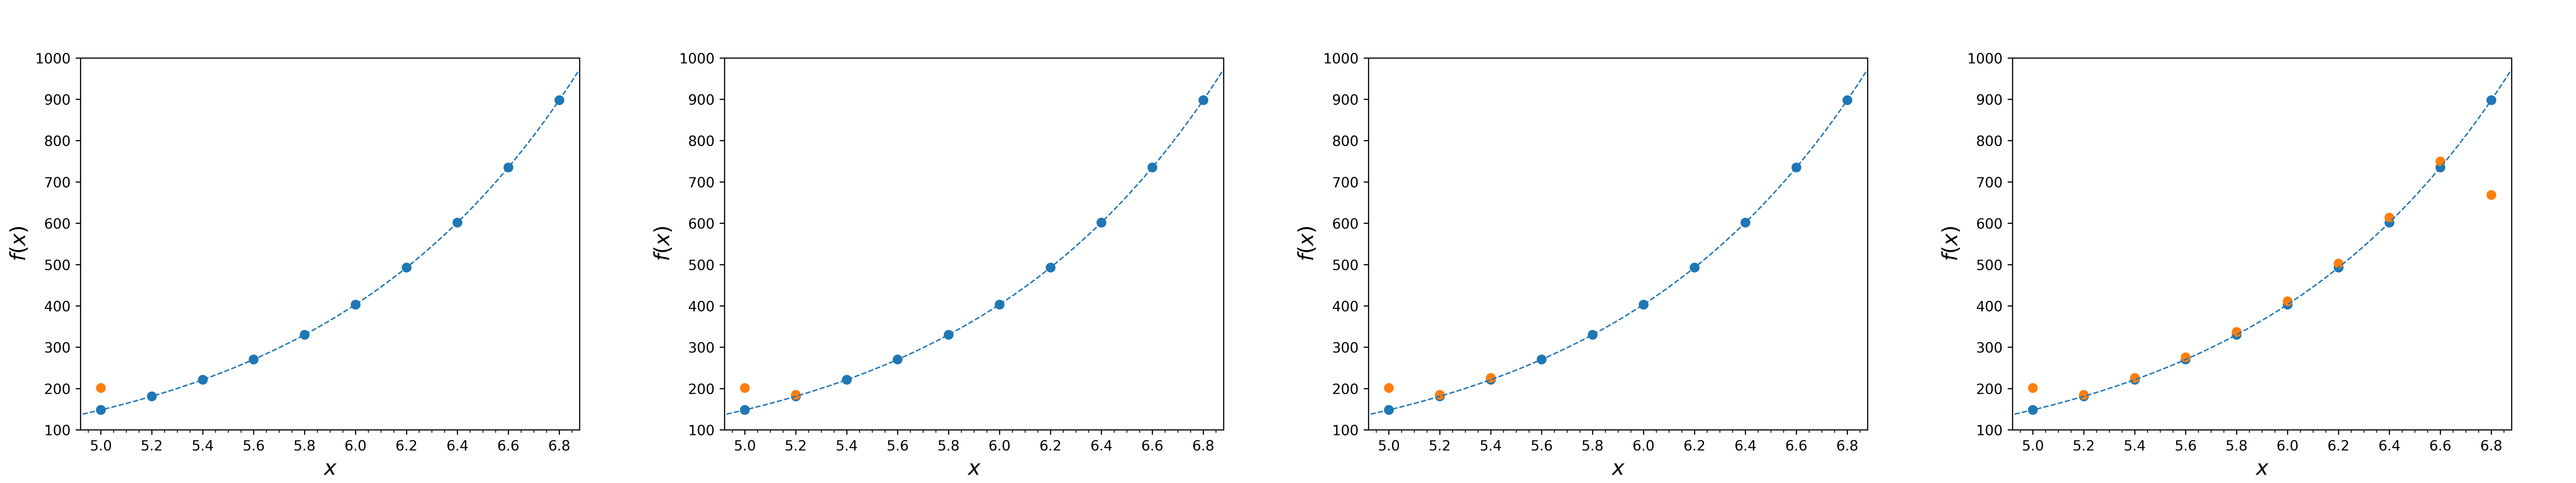
\includegraphics[width=1.0\textwidth]{figures/Fig2.png}
	\caption{Caption.}
	\label{fig:Fig2}
\end{figure*}


In Figure \ref{fig:Fig2}, one can see how the predicted values behave reasonably well for the whole range, except on the extremes. This is because the prediction at the extremes will be biased due to the knowledge along the interval. There is also an additional issue that can't be observed in the previous Figure, since our $\mathbf{x}$ values are equidistant. We can for example train the model with all our ten $x$ values, and make predictions for all values inside the studied range. The code to make all these predictions is shown here, and the results are shown in Figure \ref{fig:Fig3_1}.

\begin{lstlisting}[language=Python, caption=Code3,backgroundcolor=\color{lightgrey},keywordstyle=\color{darkgreen},commentstyle=\color{red},
showspaces=false,numbers=left,stringstyle=\color{purple}]
import math
import matplotlib.pyplot as plt
import numpy as np
from sklearn import preprocessing
from sklearn.model_selection import LeaveOneOut
from sklearn.metrics import mean_squared_error
from sklearn import neighbors
from matplotlib.ticker import (MultipleLocator)

### 1) Generate data
list_x = []
list_y = []
for i in np.arange(5, 7, 0.2):
x = i
y = math.exp(x)
list_x.append(x)
list_y.append(y)
list_x = np.array(list_x).reshape(-1, 1)
list_y = np.array(list_y)
basic_x = np.arange(4.9, 7.0, 0.01)
basic_y = [math.exp(x) for x in basic_x]

best_k = 2

### 3) Do kNN regression
X_train = np.array(list_x).reshape(-1, 1)
y_train = np.array(list_y)
X_test = np.arange(5.0, 6.81, 0.01).reshape(-1, 1)
# scale data
scaler = preprocessing.StandardScaler().fit(X_train)
X_train_scaled = scaler.transform(X_train)
X_test_scaled = scaler.transform(X_test)
knn = neighbors.KNeighborsRegressor(n_neighbors=best_k, weights='uniform')
file_name='Fig3_1.png'
label_kNN = "k-NN regression (uniform)"
# kNN regression
y_test = knn.fit(X_train_scaled, y_train).predict(X_test_scaled)
# Plot graph
plt.plot(basic_x,basic_y,color='C0',linestyle='dashed',linewidth=1)
plt.scatter(list_x, list_y,color='C0',label='$x_n$')
plt.plot(X_test, y_test,color='C1',label=label_kNN)
plt.legend()
plt.xlabel('$x$',fontsize=15)
plt.ylabel('$f(x)$',fontsize=15)
plt.xticks(np.arange(5,7,0.2))
plt.xlim(4.92,6.88)
plt.ylim(100,1000)
axes = plt.gca()
axes.xaxis.set_minor_locator(MultipleLocator(0.05))
# Save plot into png
plt.savefig(file_name,format='png',dpi=600)
plt.close()
\end{lstlisting}

\begin{figure*}[!htbp]
	\centering
	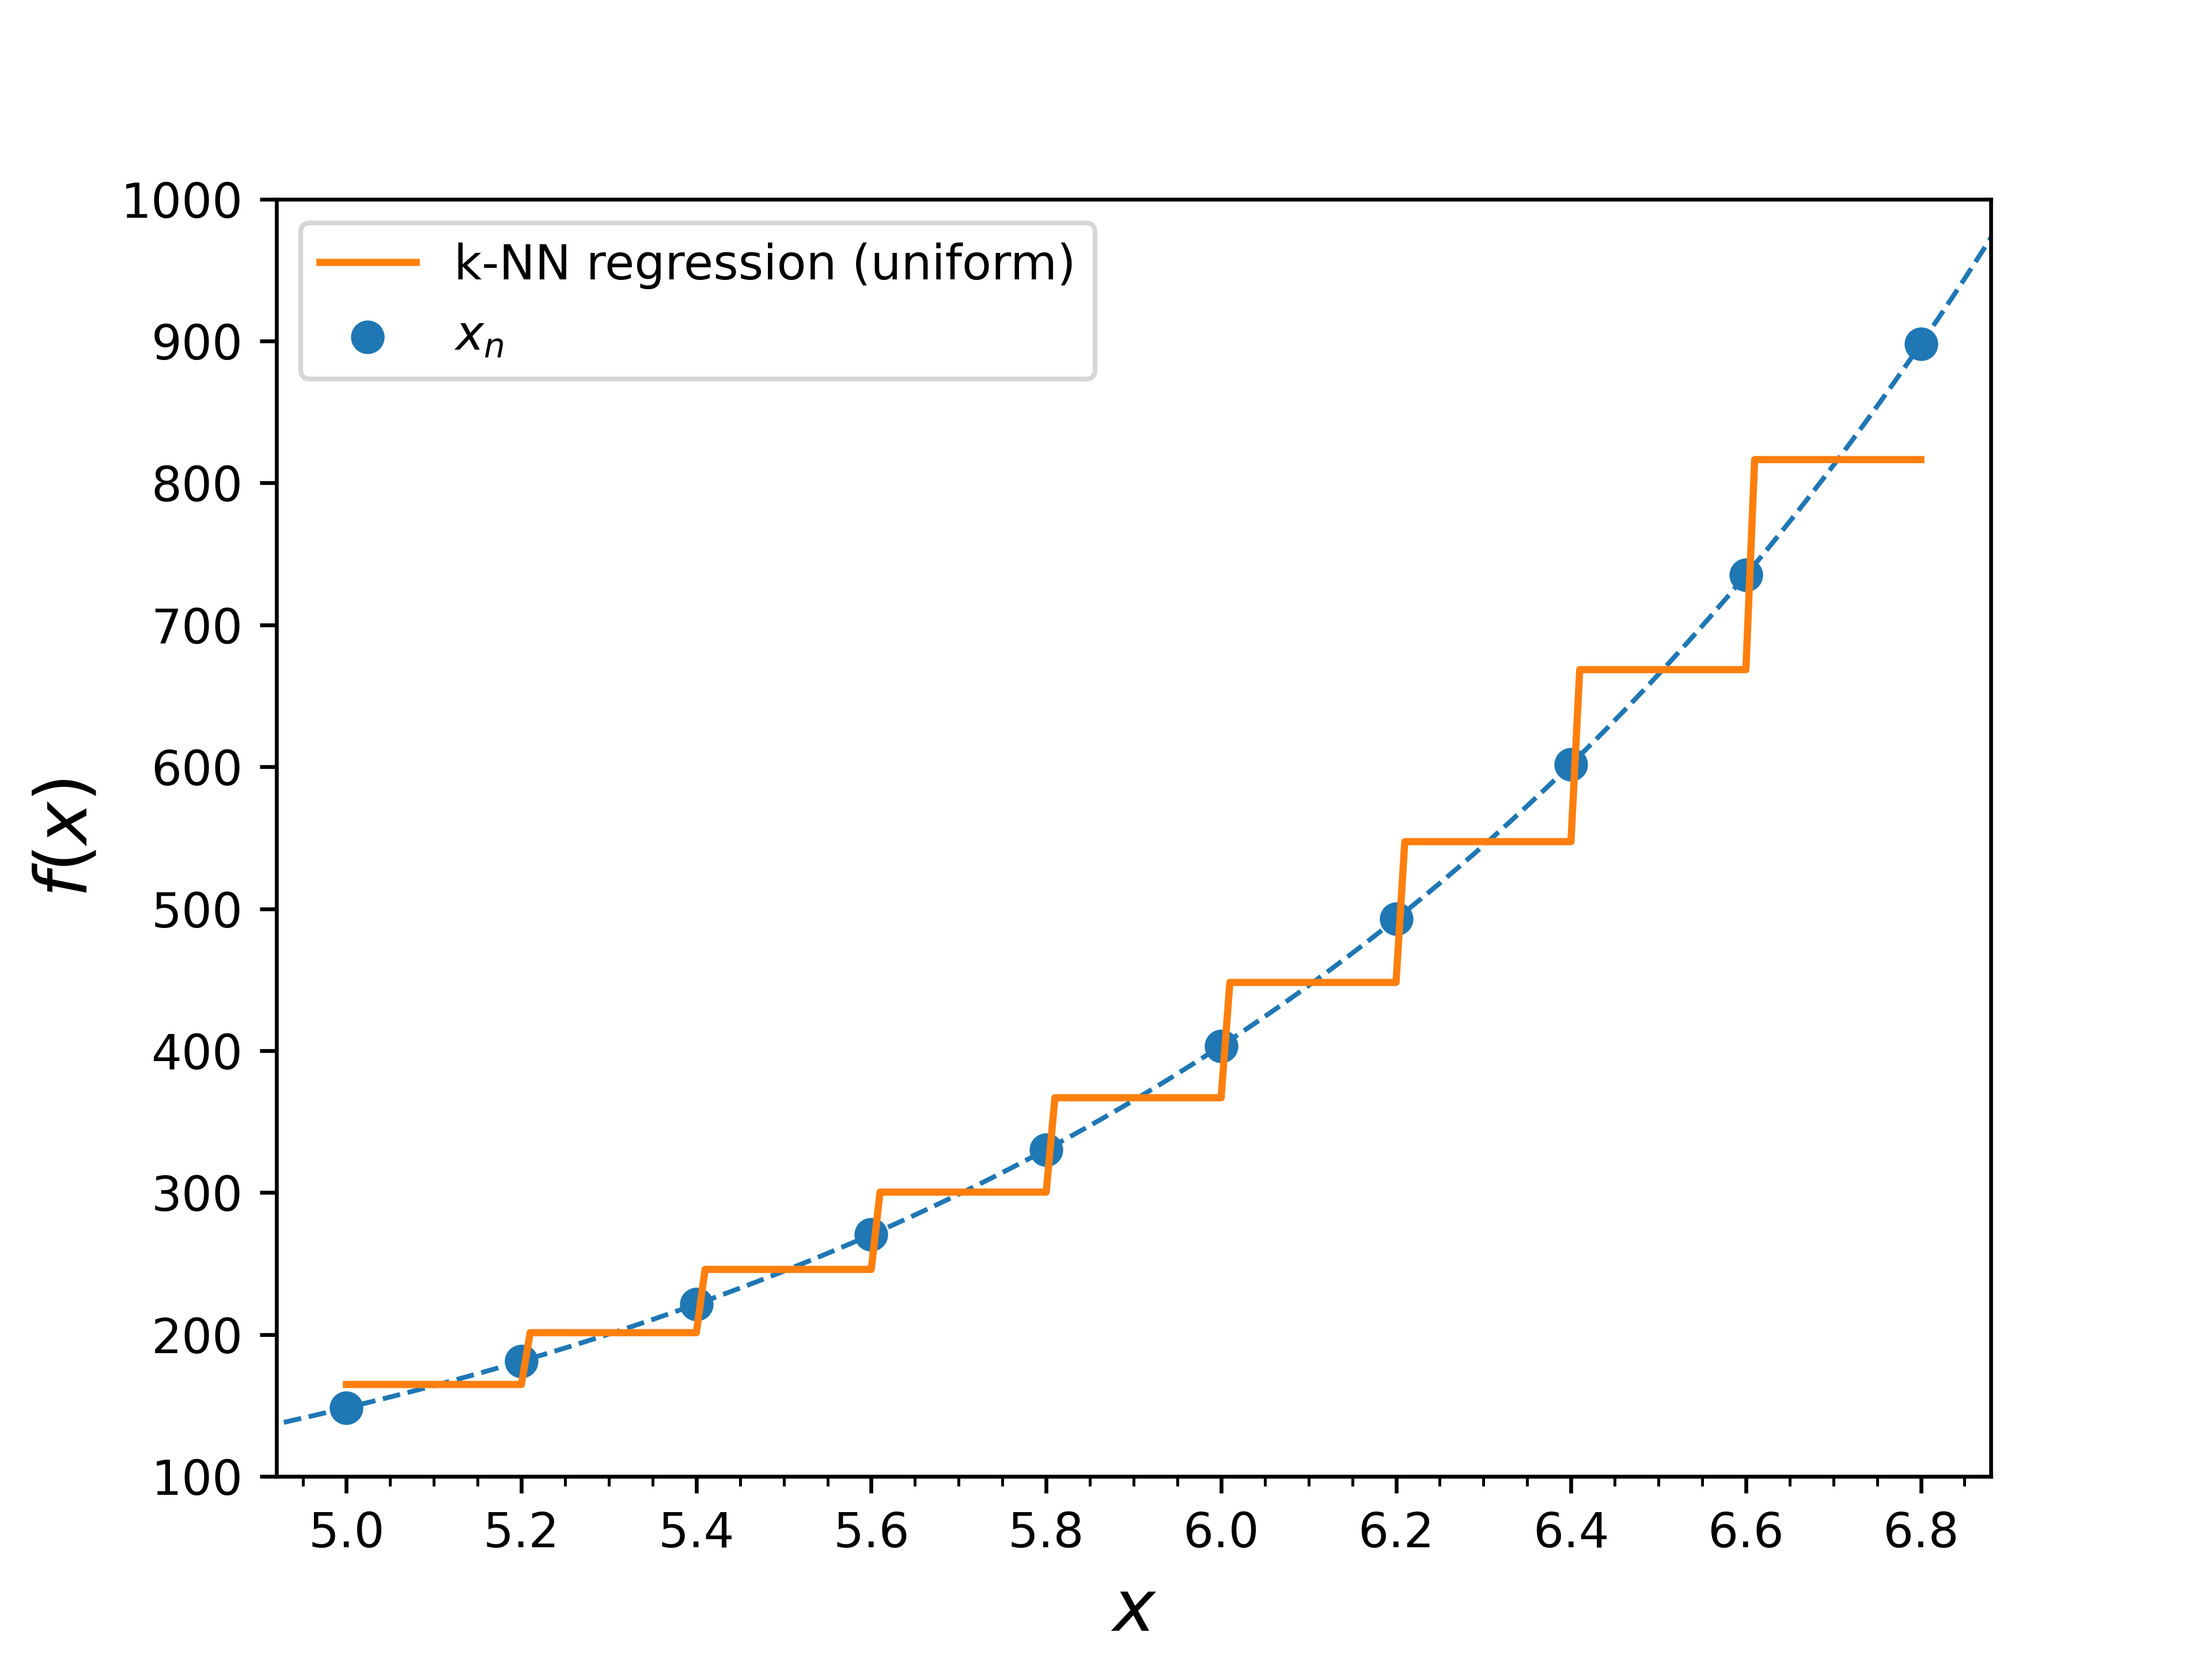
\includegraphics[width=0.75\textwidth]{figures/Fig3_1.png}
	\caption{Caption.}
	\label{fig:Fig3_1}
\end{figure*}

In Figure \ref{fig:Fig3_1} we can see how the predicted values in between the training points $x_n$ is constant, and it corresponds exactly to the average of the k nearest neighbours. This means that all k nearest neighbours have the same weight, which we specified with \textbf{weights='uniform'} (default option). However, one can clearly see how, in a case like this, it would be more accurate to give a larger weight to the neighbours that are closer.

\subsection{Different weights for nearest neighbours}
When using k-NN regression, one has to select a sensible weight function. In our case, one can see how it would be better to give a larger weight to points that are closer. This can achieved by simply using the \textbf{weights='distance'} options, that calculates weights as the inverse of the distance between the studied $i^{th}$ point and the neighbour $n$ in the training set:

\begin{align}
w_n = \frac{1}{d_n}
\label{eqn:weight_distance}
\end{align}

\noindent where $d_n$ corresponds to the Euclidean distance between $x_i$ and $x_n$. Note that one could use any other non-Euclidean metric, which might be more beneficial in other specific cases. I plan on writing a post specifically about this soon.

The result of using these new weights is shown in Figure \ref{fig:Fig3_2} and we can observe how it behaves much better for the whole studied range.

\begin{figure*}[!htbp]
	\centering
	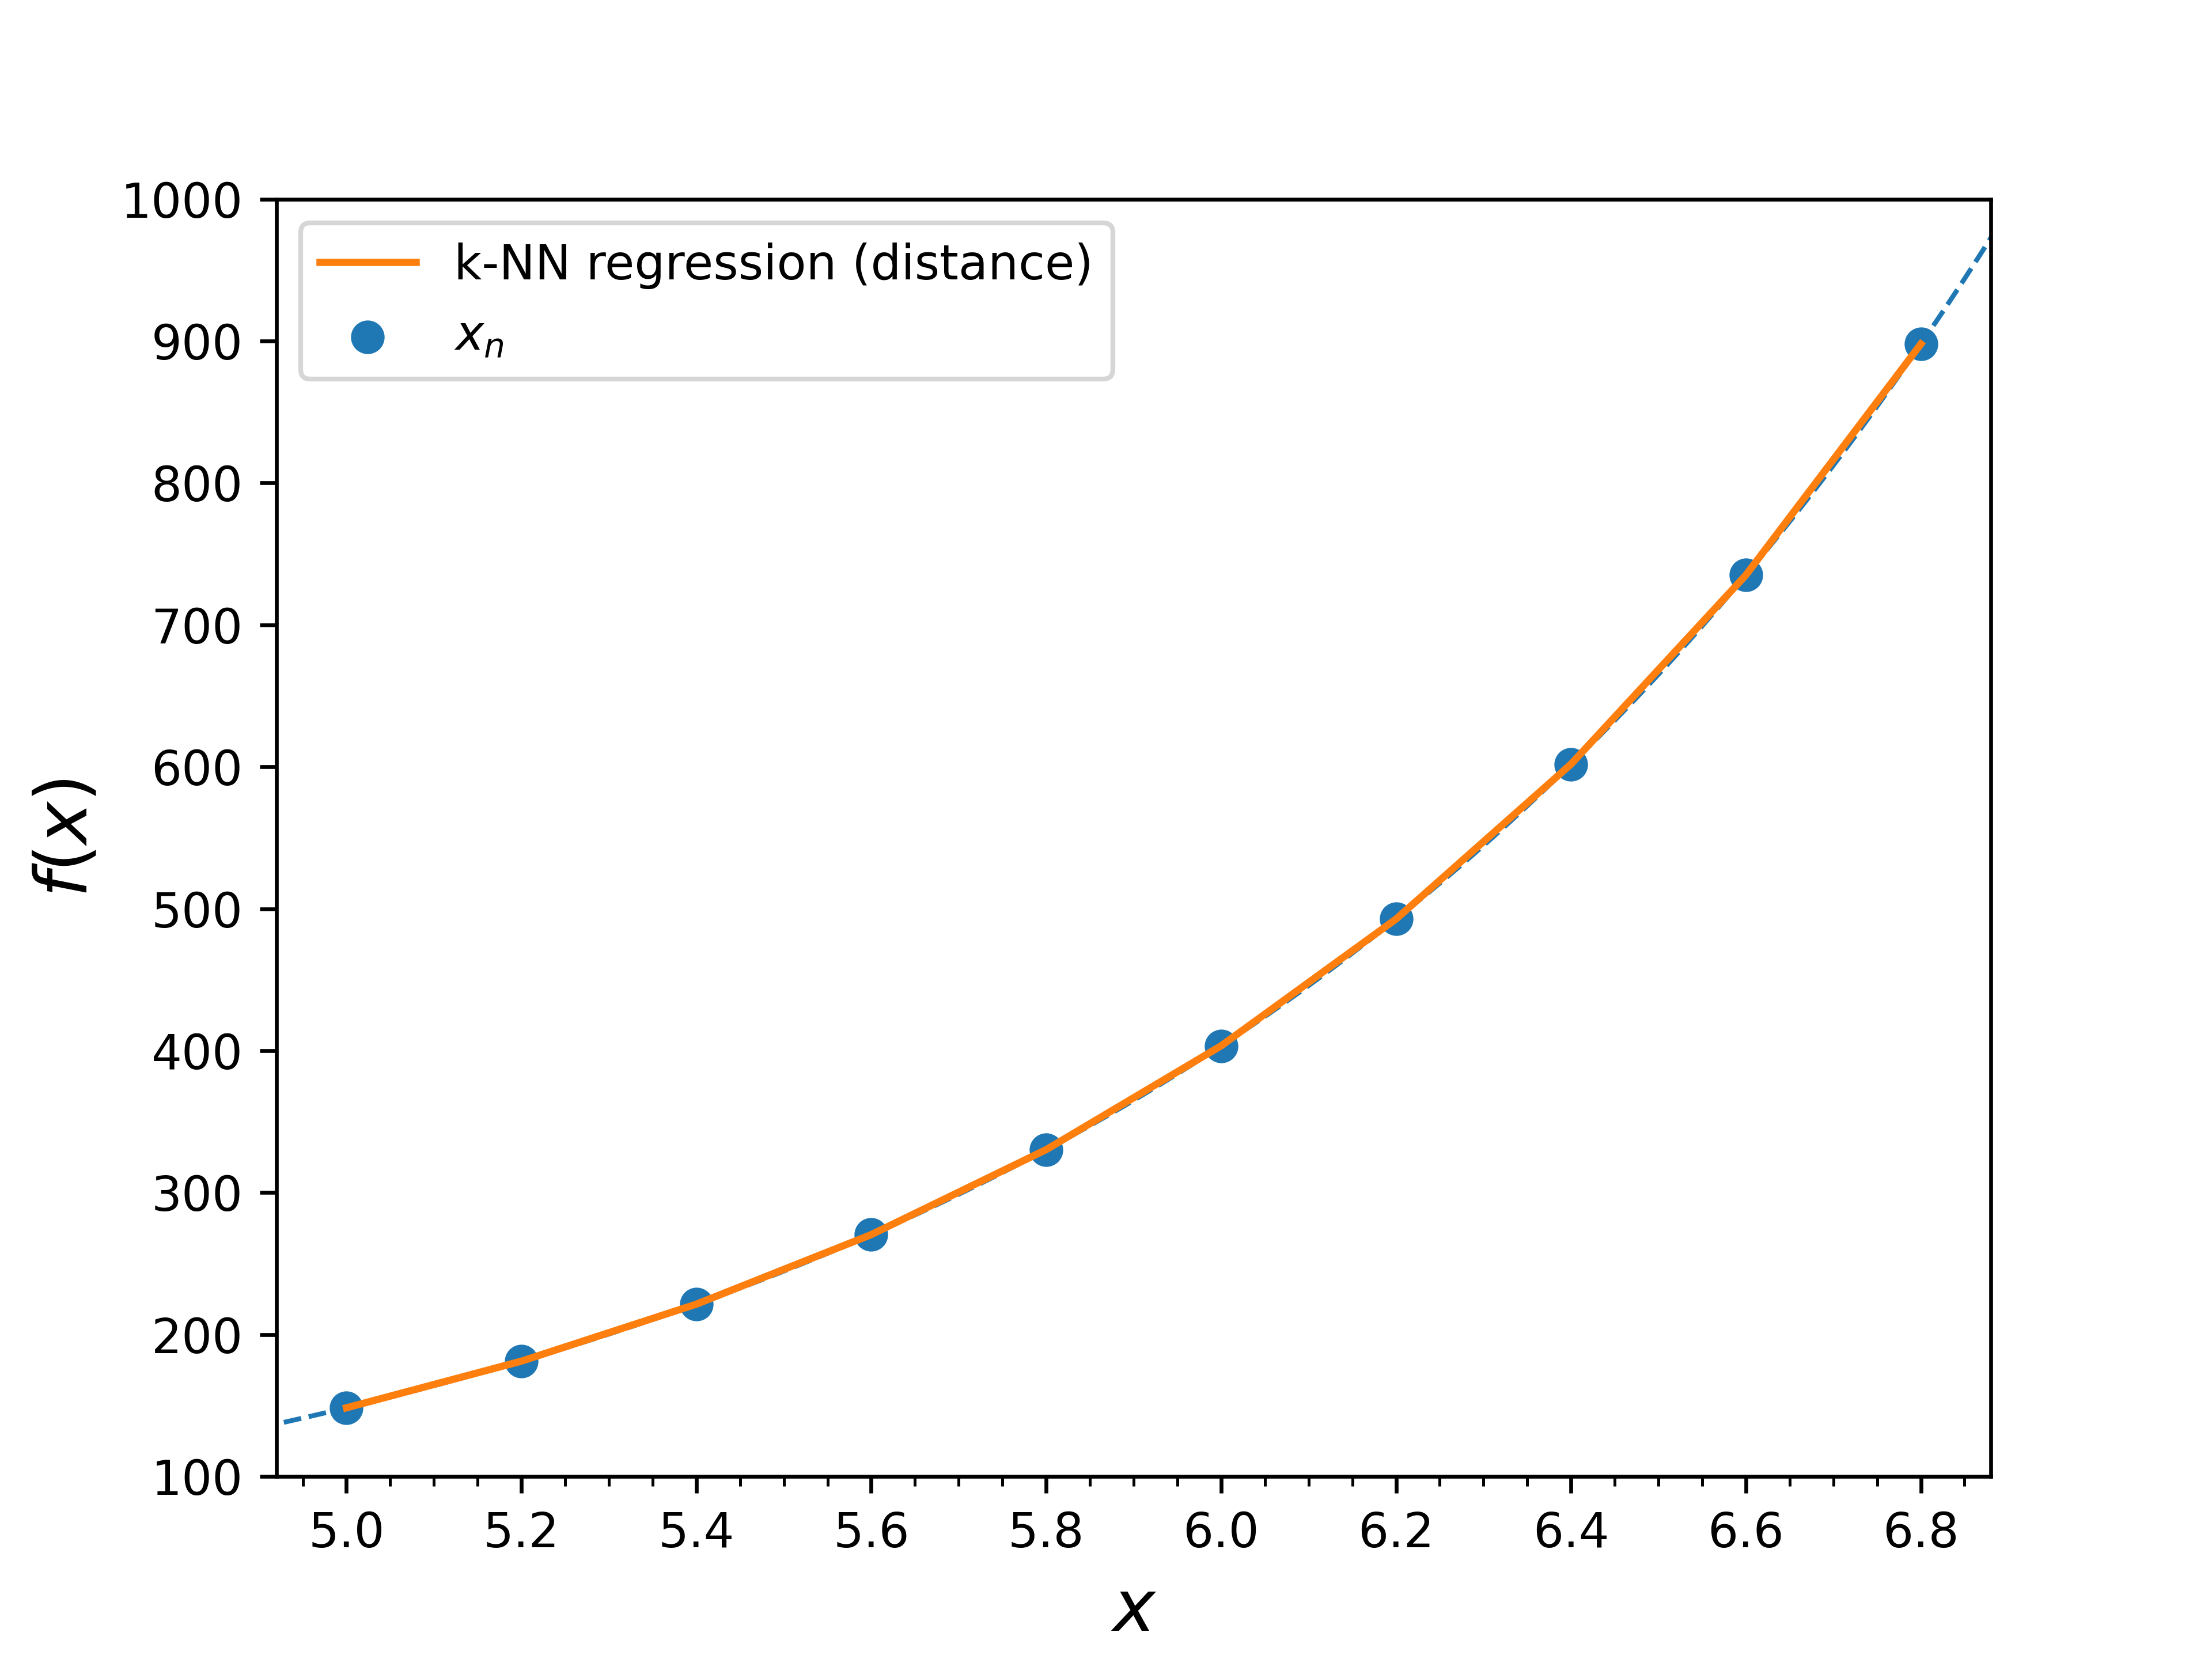
\includegraphics[width=0.75\textwidth]{figures/Fig3_2.png}
	\caption{Caption.}
	\label{fig:Fig3_2}
\end{figure*}

\section{Limitations k-NN regression}
The example that we have seen here is extremely simple, and can be seen in Figure \ref{fig:Fig3_2} how k-NN is able to make very accurate predictions within the studied range. However, one should note that even with such a simple algorithm as k-NN, one can make very accurate predictions (similar to much more sophisticated regression algorithms) in real cases in different branches of science.

However, it is worth mentioning a type of problem where k-NN performs particularly bad. This problematic task is extrapolation (i.e. predicting values that are outside the range of the training set). In general, this kind of extrapolation task is a challenge for all ML algorithms, but k-NN does particularly bad, since it purely relies in the information of neighbours in the training set, but we are in a region outside the training set.

We show in Figure \ref{fig:Fig4} how k-NN regression (with different weights) performs for the range outside the training range. We can see how k-NN totally fails to predict the exponential behaviour expected outside the training range and it simply returns the weighted average value of the two nearest neighbours.

\begin{figure*}[!htbp]
	\centering
	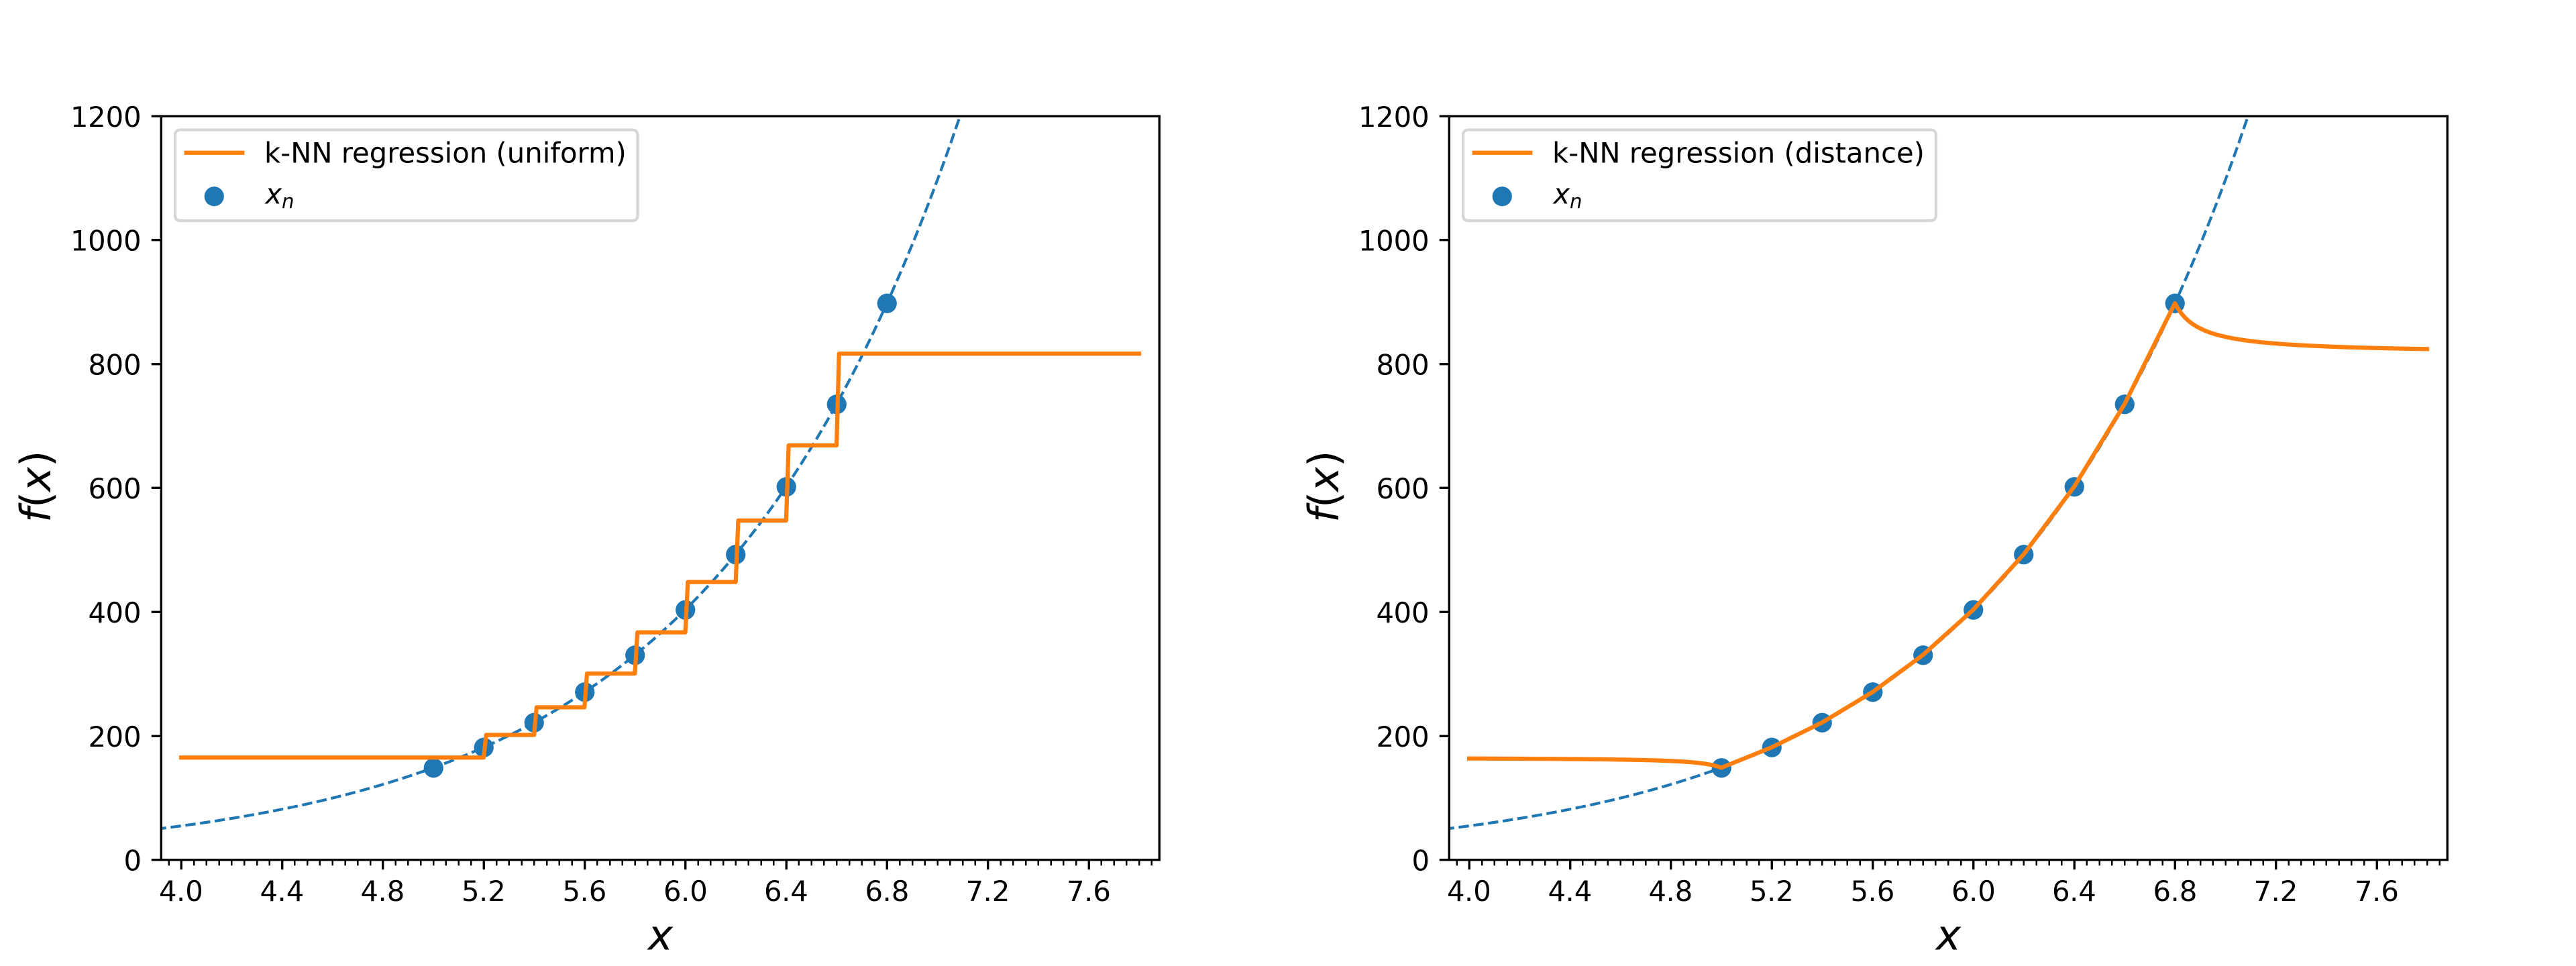
\includegraphics[width=1.0\textwidth]{figures/Fig4.png}
	\caption{Caption.}
	\label{fig:Fig4}
\end{figure*}

The code used to generate Fig \ref{fig:Fig4} is shown below.

\begin{lstlisting}[language=Python, caption=Code3,backgroundcolor=\color{lightgrey},keywordstyle=\color{darkgreen},commentstyle=\color{red},
showspaces=false,numbers=left,stringstyle=\color{purple}]
import math
import matplotlib.pyplot as plt
import numpy as np
from sklearn import preprocessing
from sklearn.model_selection import LeaveOneOut
from sklearn.metrics import mean_squared_error
from sklearn import neighbors
from matplotlib.ticker import (MultipleLocator)

### 1) Generate data
list_x = []
list_y = []
for i in np.arange(5, 7, 0.2):
x = i
y = math.exp(x)
list_x.append(x)
list_y.append(y)
list_x = np.array(list_x).reshape(-1, 1)
list_y = np.array(list_y)
basic_x = np.arange(3.9, 8.0, 0.01)
basic_y = [math.exp(x) for x in basic_x]

best_k = 2

### 4) Do kNN regression extrapolation
X_train = np.array(list_x).reshape(-1, 1)
y_train = np.array(list_y)
X_test = np.arange(4.0, 7.81, 0.01).reshape(-1, 1)
# scale data
scaler = preprocessing.StandardScaler().fit(X_train)
X_train_scaled = scaler.transform(X_train)
X_test_scaled = scaler.transform(X_test)
################################################################################
############# UNIFORM #############
#knn = neighbors.KNeighborsRegressor(n_neighbors=best_k, weights='uniform')
#file_name='Fig4_1.png'
#label_kNN = "k-NN regression (uniform)"
############# DISTANCE #############
knn = neighbors.KNeighborsRegressor(n_neighbors=best_k, weights='distance')
file_name='Fig4_2.png'
label_kNN = "k-NN regression (distance)"
################################################################################
# kNN regression
y_test = knn.fit(X_train_scaled, y_train).predict(X_test_scaled)
# Plot graph
plt.plot(basic_x,basic_y,color='C0',linestyle='dashed',linewidth=1)
plt.scatter(list_x, list_y,color='C0',label='$x_n$')
plt.plot(X_test, y_test,color='C1',label=label_kNN)
plt.legend()
plt.xlabel('$x$',fontsize=15)
plt.ylabel('$f(x)$',fontsize=15)
plt.xticks(np.arange(4,8,0.4))
plt.xlim(3.92,7.88)
plt.ylim(0,1200)
axes = plt.gca()
axes.xaxis.set_minor_locator(MultipleLocator(0.05))
# Save plot into png
plt.savefig(file_name,format='png',dpi=600)
plt.close()
\end{lstlisting}

\end{document}

